%!TEX program = xelatex
\documentclass{beamer}

\usepackage[english]{babel}

\usepackage{graphicx,hyperref,url, materialbeamer}
\usepackage{braket}
%\usepackage{euler}
\usepackage{listings}

\usepackage{multirow}
\usepackage{changepage}
\usepackage{ragged2e}

\makeatletter
\newcommand{\jtemize}[1][]{%
	\beamer@ifempty{#1}{}{\def\beamer@defaultospec{#1}}%
	\ifnum \@itemdepth >2\relax\@toodeep\else
	\advance\@itemdepth\@ne
	\beamer@computepref\@itemdepth% sets \beameritemnestingprefix
	\usebeamerfont{itemize/enumerate \beameritemnestingprefix body}%
	\usebeamercolor[fg]{itemize/enumerate \beameritemnestingprefix body}%
	\usebeamertemplate{itemize/enumerate \beameritemnestingprefix body begin}%
	\list
	{\usebeamertemplate{itemize \beameritemnestingprefix item}}
	{\def\makelabel##1{%
			{%
				\hss\llap{{%
						\usebeamerfont*{itemize \beameritemnestingprefix item}%
						\usebeamercolor[fg]{itemize \beameritemnestingprefix item}##1}}%
			}%
		}%
	}
	\fi%
	\beamer@cramped%
	\justifying% NEW
	%\raggedright% ORIGINAL
	\beamer@firstlineitemizeunskip%
}
\def\endjtemize{\ifhmode\unskip\fi\endlist%
	\usebeamertemplate{itemize/enumerate \beameritemnestingprefix body end}
	\ifnum \@itemdepth >1
	\vfil
	\fi%  
}
\makeatother


\setbeamercovered{transparent}

\usefonttheme{}

% The title of the presentation:
%  - first a short version which is visible at the bottom of each slide;
%  - second the full title shown on the title slide;
\title[WFCNet for FPAR]{Aid of WFCNet\\for FPAR Task}

% Optional: a subtitle to be dispalyed on the title slide
\subtitle{Project Description}

% The author(s) of the presentation:
%  - again first a short version to be displayed at the bottom;
%  - next the full list of authors, which may include contact information;
\author[Nicolò Bertozzi, Francesco Bianco Morghet]{Nicolò Bertozzi, Francesco Bianco Morghet} 
  
%\titlegraphic{\includegraphics[width=\textwidth]{atac-logo}}

% The institute:
%  - to start the name of the university as displayed on the top of each slide
%    this can be adjusted such that you can also create a Dutch version
%  - next the institute information as displayed on the title slide
\institute[Politecnico di Torino]{
Machine Learning and Deep Learning\\
Master Degree in Data Science Engineering\\
Politecnico di Torino}

% Add a date and possibly the name of the event to the slides
%  - again first a short version to be shown at the bottom of each slide
%  - second the full date and event name for the title slide
\date[2$^{nd}$ Semester]{
 2$^{nd}$ Semester | 13 July 2020}

\providecommand{\di}{\mathop{}\!\mathrm{d}}
\providecommand*{\der}[3][]{\frac{d\if?#1?\else^{#1}\fi#2}{d #3\if?#1?\else^{#1}\fi}} 
 \providecommand*{\pder}[3][]{% 
    \frac{\partial\if?#1?\else^{#1}\fi#2}{\partial #3\if?#1?\else^{#1}\fi}% 
  }

\begin{document}

\begin{frame}
  \titlepage
\end{frame}

\begin{frame}
  \frametitle{Table of Contents}
  \tableofcontents
\end{frame}

\section{Introduction}

\begin{frame}
\frametitle{Overview} 
  \tableofcontents[currentsection]
\end{frame}

\begin{frame}
\frametitle{Introduction 1/4}
Goal:
\begin{itemize}
\item Record videos with the same cameraman's point of view;
\item Recognize the actions performed by the subject;
\end{itemize}
\end{frame}

\begin{frame}
\frametitle{Introduction 2/4}
\begin{columns}
\column{0.5\textwidth}
Interested Areas:
\begin{itemize}
\item Android intelligence;
\item Autonomous driving;
\item Surveillance;
\item Loyalizing users' experience;
\end{itemize}
\column{0.5\textwidth}
\begin{figure}
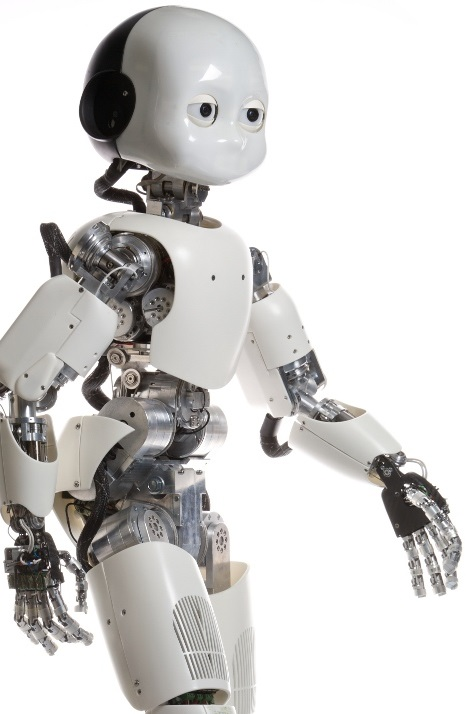
\includegraphics[width=0.8\textwidth]{../schemi/icub}
\end{figure}
\end{columns}
\end{frame}

\begin{frame}
\frametitle{Introduction 3/4}
Issues:
\begin{itemize}
\item Small datasets;
\item Presence of \textbf{parts of the cameraman's body} in the video;
\item The action \textbf{must be represented} by a \emph{verb + noun};
\end{itemize}
\end{frame}

\begin{frame}
\frametitle{Introduction 4/4}
Solutions:
\begin{itemize}
\item Sales of \textbf{wearable devices};
\item Incrementing chance of \textbf{having at hand a camera};
\item Incrementing number of \textbf{images taken every day} \cite{photos};
\item Deeper neural networks;
\end{itemize}
\end{frame}

\section{Dataset}

\begin{frame}
\frametitle{Overview} 
  \tableofcontents[currentsection]
\end{frame}

\begin{frame}
\frametitle{Dataset}

\begin{columns}[c]
	\begin{column}{.5\textwidth}
		GTEA-61:
		\begin{itemize}
			\item First person point of view;
			\item 61 classes of \textit{verb+noun};
			\item 4 subjects;
			\item Most clips 1.5s to 4s long;
		\end{itemize}
	\end{column}
	\begin{column}{.5\textwidth}
		\begin{figure}
			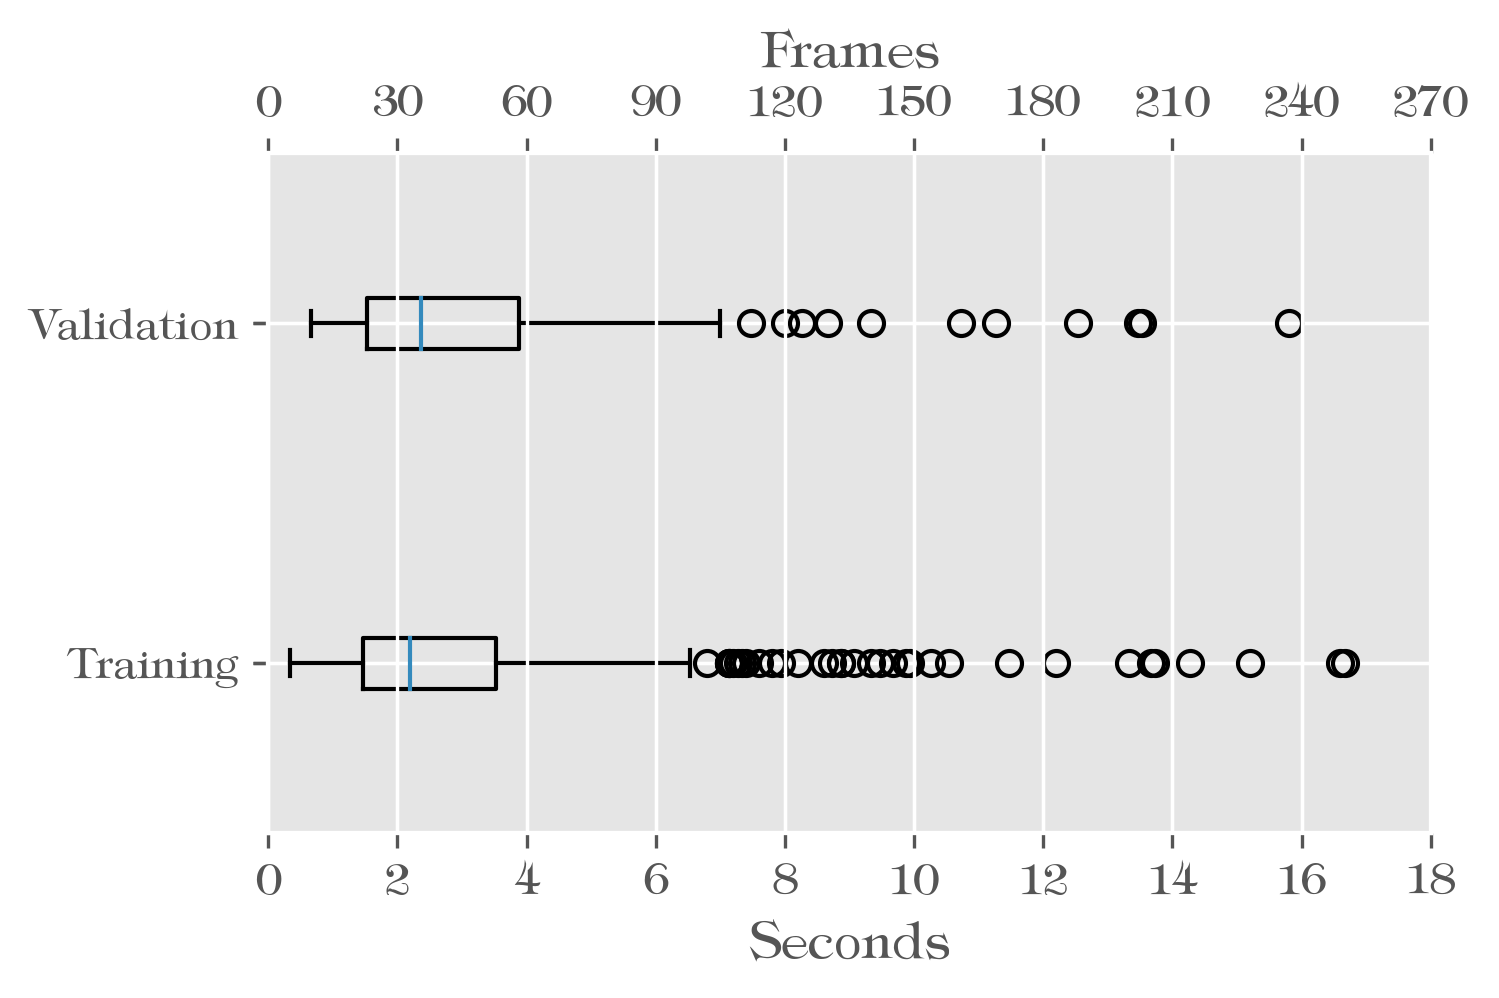
\includegraphics[width=\textwidth]{../schemi/GTEA61_boxplot.png}
		\end{figure}
	\end{column}
\end{columns}

\vspace{24pt}
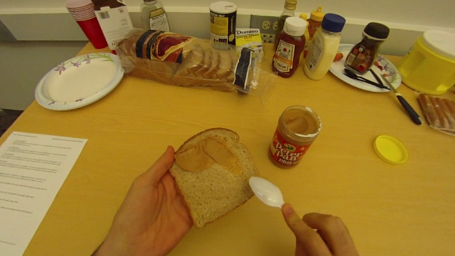
\includegraphics[width=.22\textwidth]{../schemi/frame_1.png} \hfill
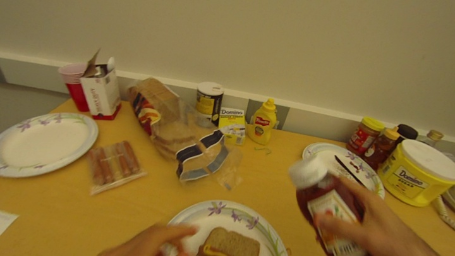
\includegraphics[width=.22\textwidth]{../schemi/frame_2.png} \hfill
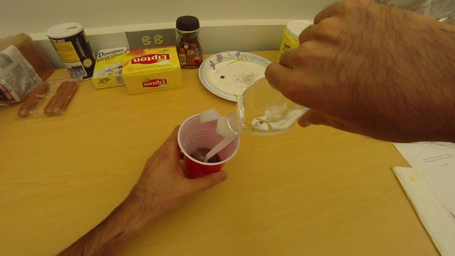
\includegraphics[width=.22\textwidth]{../schemi/frame_3.png} \hfill
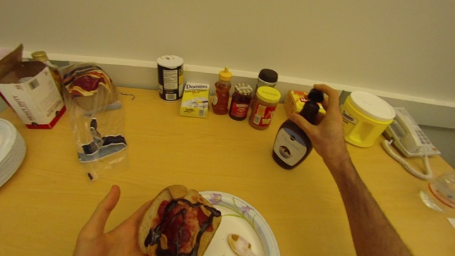
\includegraphics[width=.22\textwidth]{../schemi/frame_4.png}

\end{frame}
      
\section{Related Works}

\begin{frame}
\frametitle{Overview} 
  \tableofcontents[currentsection]
\end{frame}

\begin{frame}
\frametitle{Two Stream Approach 1/2}
\begin{columns}
\column{0.6\textwidth}
Main characteristics:
\begin{jtemize}
\item \textbf{Two networks} with separate \textbf{CNNs}: one to \textbf{extract features} from RGB images and one to \textbf{extract features} from warped optical flow frames;
\item \textbf{ConvLSTM} in the RGB network to take into account the \textbf{temporal dependencies};
\item Linear \textbf{classifier} to \textbf{join} the two networks;
\end{jtemize}
\column{0.4\textwidth}
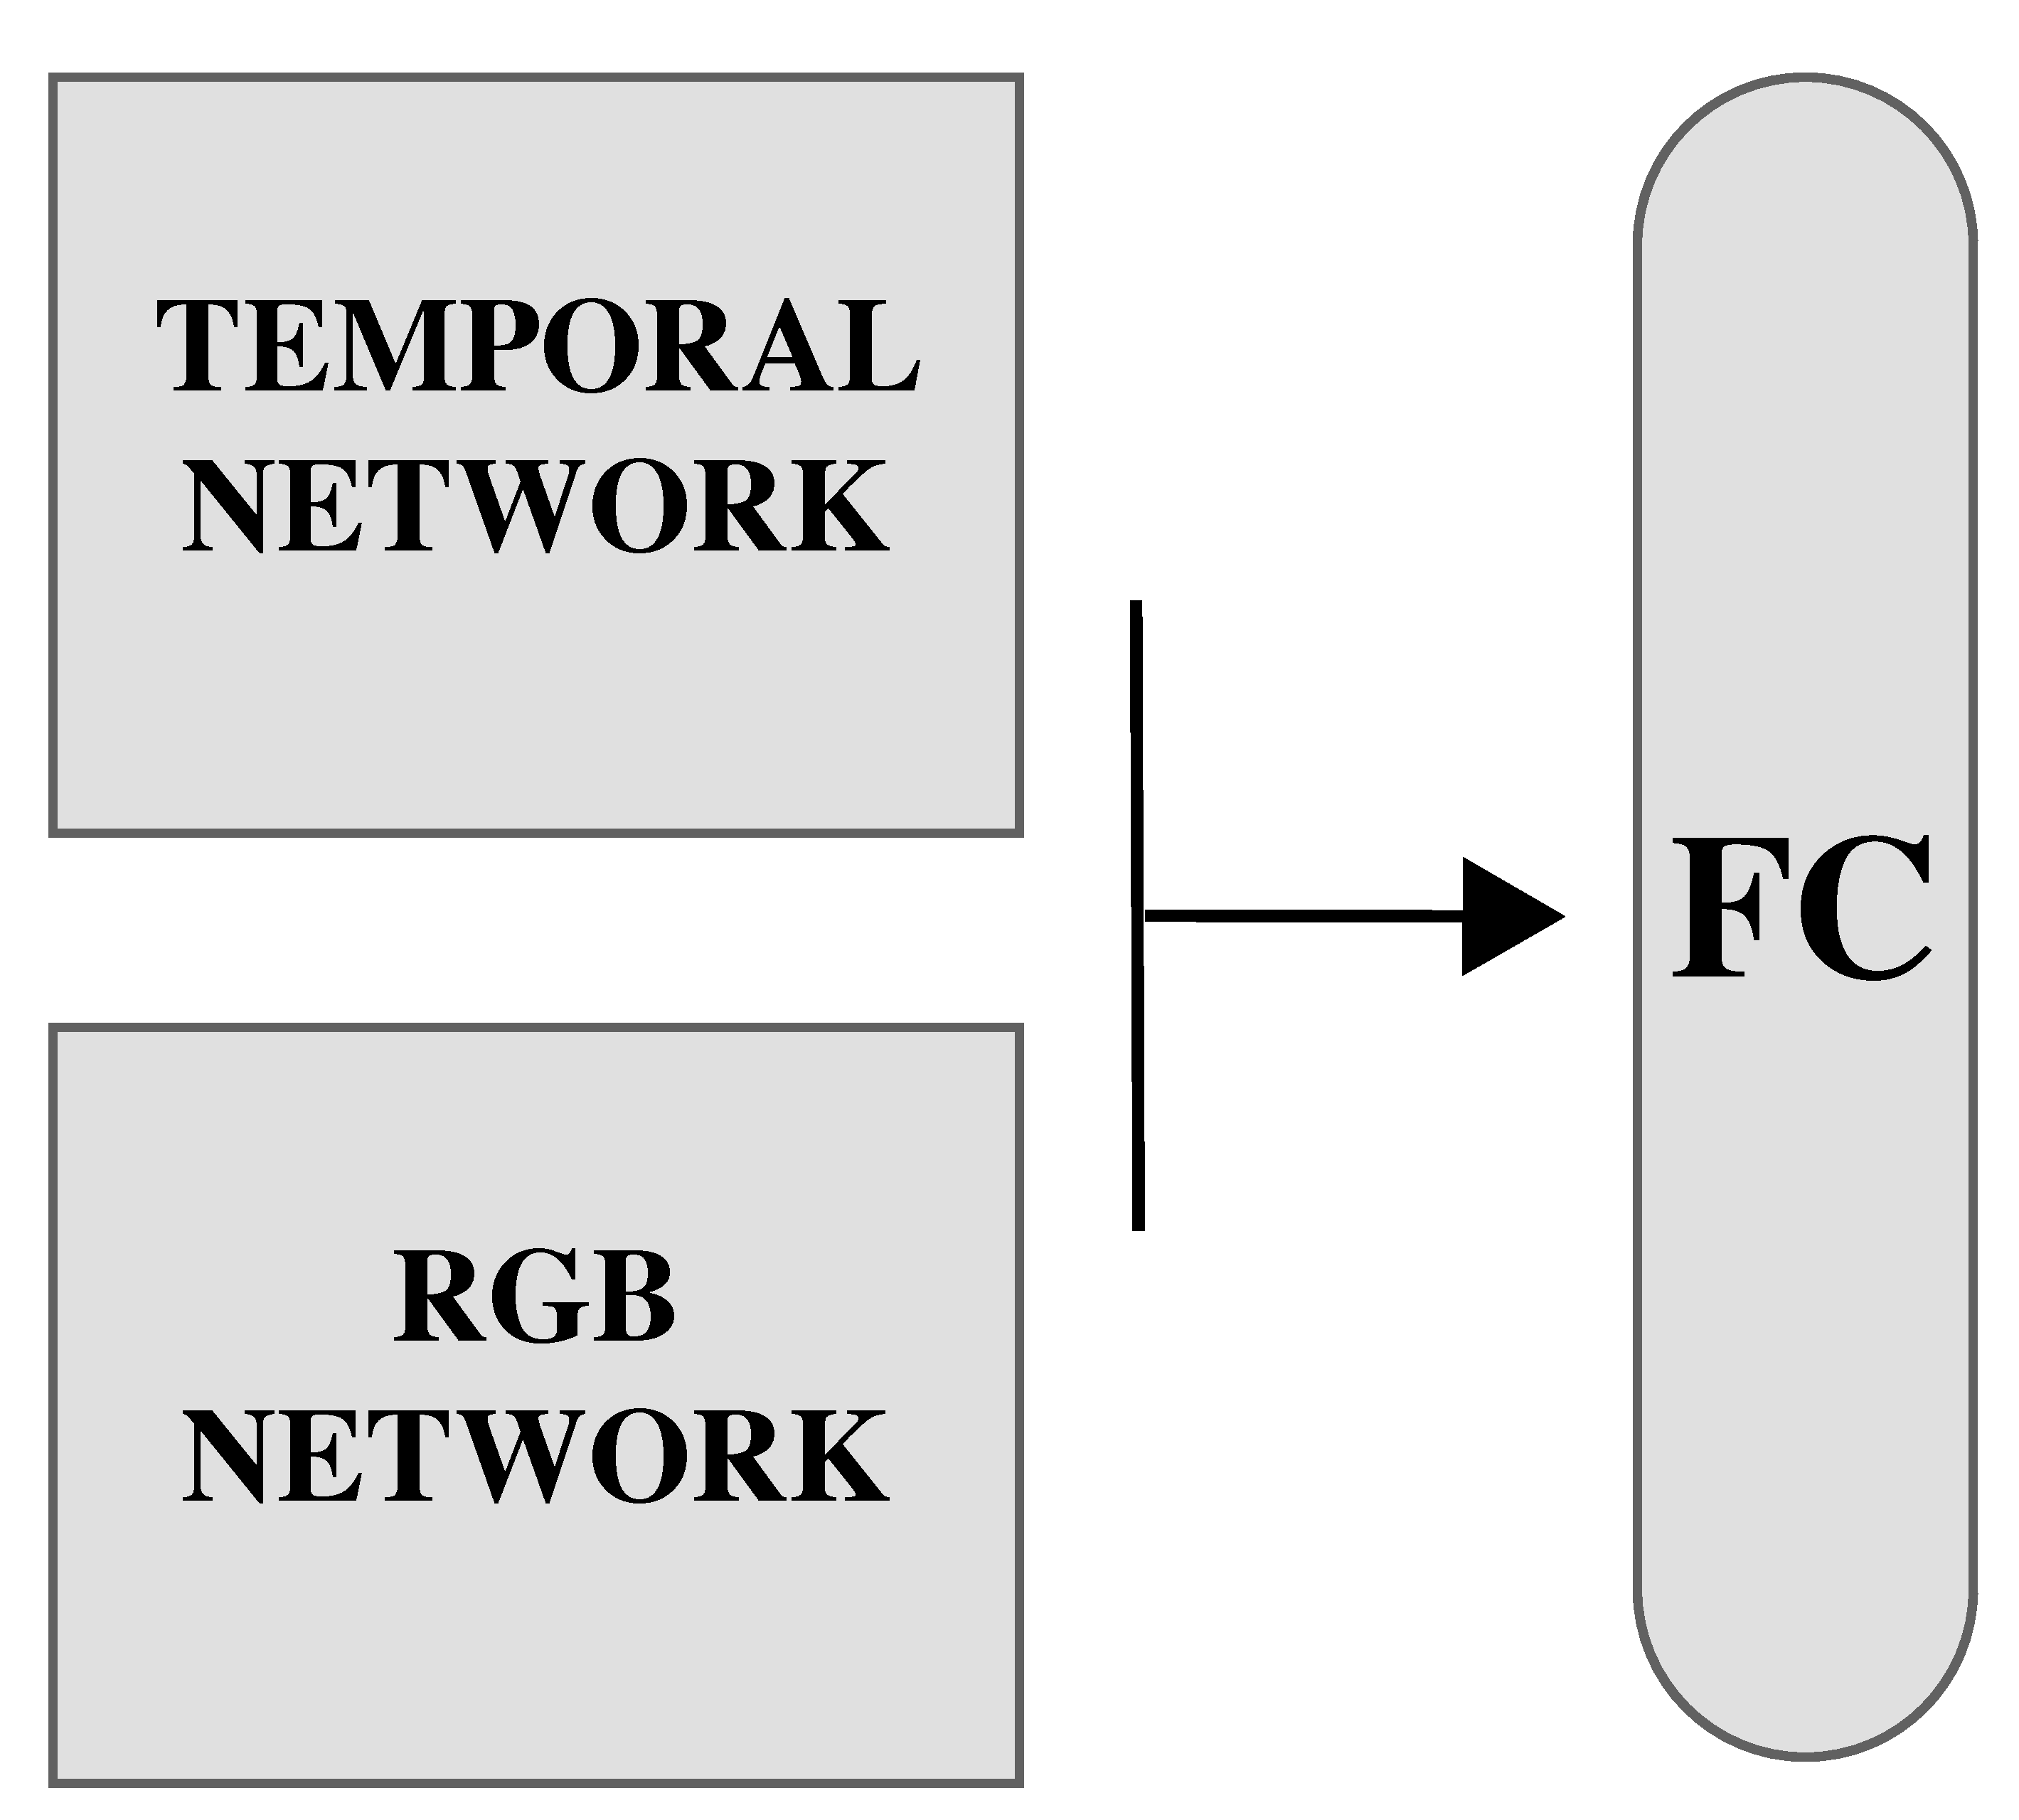
\includegraphics[width=\textwidth]{../schemi/contribution}
\end{columns}
\end{frame}

\begin{frame}
\frametitle{Two Stream Approach 2/2}
Issue:
\begin{itemize}
\item The correlation and the \textbf{mutual influence} between motion and appearance information is \textbf{not taken into account};
\end{itemize}
Possible solution:
\begin{itemize}
\item Implementing a single network with an auxiliary \textbf{self supervised task};
\end{itemize}
\end{frame}

\begin{frame}
\frametitle{Motion Segmentation Task 1/2}

Features:
\begin{itemize}
\item Each \textbf{feature map} is forwarded to an \textbf{auxiliary branch} with a convolutional and a FC layer;
\item \textbf{IDT} as ground truth: image which indicates if a \textbf{pixel is moving or not}, net to the camera motion;
\item \textbf{Pixel-per-pixel loss} between the predicted motion map and the IDT;
\end{itemize}

\end{frame}

\begin{frame}
\frametitle{Motion Segmentation Task 2/2}
\begin{adjustwidth}{-1.75em}{-1.75em}


\begin{itemize}
	\item Both tasks are jointly trained by minimising single loss:
	\begin{center}
	${\displaystyle {\mathcal{L} = \mathcal{L}_{main} + \alpha \mathcal{L}_{ms} \hspace{10pt} , \hspace{10pt} \alpha \in \Re} }$
	\end{center}
	
	\item Loss of classification task:
	
	\begin{center}
	\begin{tabular}{cr}
		\multirow{2}{*}{$ {\displaystyle \mathcal{L}_{main} = -\sum_i^N{y_i \log (p(x_i))} }$} 
		& $y_i = [0 \dots 1 \dots 0]$ \\
		& $ p(x_i) = \frac{1}{\sum_j e^{f_j}} [ e^{f_0} \dots e^{f_c} ]$
	\end{tabular}
	\end{center}

	{\scriptsize $x_i$ sample, $y_i$ label, $f_j$ output neuron for class $j$ }

	\item Loss of motion segmentation task:
	
	\begin{minipage}{.6\textwidth}
		CLF: $ {\displaystyle \mathcal{L}_{ms} = -\sum_i^N\sum_t^T\sum_s^S{m_{i,t,s} \log (l_{i,t,s}) } }$ \\
		REG: $ {\displaystyle \mathcal{L}_{ms} = -\sum_i^N\sum_t^T\sum_s^S{(m_{i,t,s}' - l_{i,t,s}')^2 } }$
	\end{minipage}%
	\begin{minipage}{.4\textwidth}
		\begin{flushright}
		${ \scriptstyle m_{i,t,s} \in \{ [1, 0], [0, 1] \} }$ 
		${ \scriptstyle m_{i,t,s}' \in \{ 0, 1 \} }$
		${ \scriptstyle l_{i,t,s} = \left [ \frac{e^{f_{s_0}(i, t)}}{\sum_j e^{f_{s_j}(i, t)}}, \frac{e^{f_{s_1}(i, t)}}{\sum_j e^{f_{s_j}(i, t)}} \right ] }$ \\
		${ \scriptstyle l_{i,t,s}' =  .5 \tanh (f_{s_0}(i, t) + f_{s_1}(i, t)) + .5 }$
		\end{flushright}
	\end{minipage}

	{\scriptsize $i$ sample, $t$ time-step, $s$ spatial location, $m$ mmap, $l$ predicted mmap, \\ \vspace*{-5pt} $f_{s_j}$ output neuron for spatial location $s$ and pixel value $j = 0|1$}

	
\end{itemize}

\end{adjustwidth}
\end{frame}

\begin{frame}
\frametitle{CAMs Visualizations}

\begin{figure}
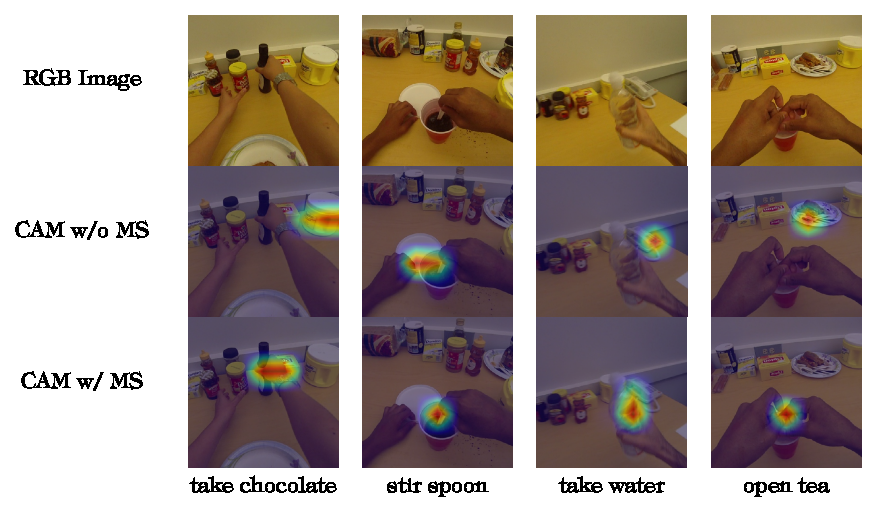
\includegraphics[width=\textwidth]{../schemi/cams_img}
\end{figure}

\end{frame}

\begin{frame}
\frametitle{Attention Mechanism 1/2}

Features:
\begin{itemize}
\item \textbf{Focusing} the recognition on the \textbf{most important parts} of the video;
\item \textbf{Discarding} the regions with \textbf{low importance};
%\item The temporal flow information, i.e \textbf{the motion}, \textbf{is not included} in the mechanism; % No questo non vale per il nostro
\end{itemize}

\end{frame}

\begin{frame}
\frametitle{Attention Mechanism 2/2}

\begin{columns}[t]
	\begin{column}{0.5\textwidth}
		Attention mechanism in Ego-RNN:
		\vspace{6pt}
		{ \scriptsize
		\begin{enumerate}
			\item Find best neuron of hidden fc layer:
			${{\text{argmax}}_c (\sum_l(\text{avgpool}_i(f_i(l)) \cdot w_l^c) + b^c )}$
			\item Compute CAM for all spatial locations: 
			${\text{CAM}_c(i) = \sum_l w_l^c f_l(i)}$
			\item Compute features with spatial attention: \\
			$f_{SA} = CAM' \odot f $ \\ $CAM'(i) =  \frac{e^{CAM(i)}}{\sum_i e^{CAM(i)}}$
		\end{enumerate}
		}
	\end{column} %
	\begin{column}{0.5\textwidth}
		Proposed simpler attention mechanism:
		\vspace{6pt}
		{ \scriptsize
			\begin{enumerate}
				\item Compute AM for all spatial locations: 
				${\text{AM}(i) = \sum_l w_l f_l(i)}$
				\item Compute features with spatial attention: \\
				$f_{SA} = AM' \odot f $ \\ $ AM'(i) =  \frac{e^{AM(i)}}{\sum_i e^{AM(i)}}$
			\end{enumerate}
		}
	\end{column}
\end{columns}

\vfill

{\scriptsize $i$ spatial location index, $l$ output feature map index, $c$ hidden neuron index \\ 
$f_l(i)$ backbone $l$-th output feature map at spatial location $i$, \\
$w_l^c$ $l$-th weight of $c$-th neuron, $b^c$ bias of $c$-th neuron, \\  
\vspace{-4pt}
$w_l$ $l$-th weight of linear classifier}


\end{frame}

\section{Proposed Methods}

\begin{frame}
\frametitle{Overview} 
	\tableofcontents[currentsection]
\end{frame}

\begin{frame}
\frametitle{WFCNet 1/2}

Network's composition:
\begin{itemize}
\item \textbf{Resnet-like architecture};
\item \textbf{Macro blocks} execute directly the \textbf{downsampling} or the \textbf{upsampling};
\item \textbf{Downsampling as convolutional filters} which maintain the pros of residual blocks;
\item \textbf{Upsampling as neighbour resize} which performs better than transpose convolution;
\item Finally the \textbf{activation function} with sigmoid and the \textbf{normalisation} with mean and std of ImageNet are applied;
\end{itemize}
 
\end{frame}

\begin{frame}
\frametitle{WFCNet 2/2}

\begin{figure}
\includegraphics[width=\textwidth]{../schemi/wfcnet_esploso}
\end{figure}
 
\end{frame}

\begin{frame}
\frametitle{Training WFCNet 1/2}

\begin{figure}
\centering
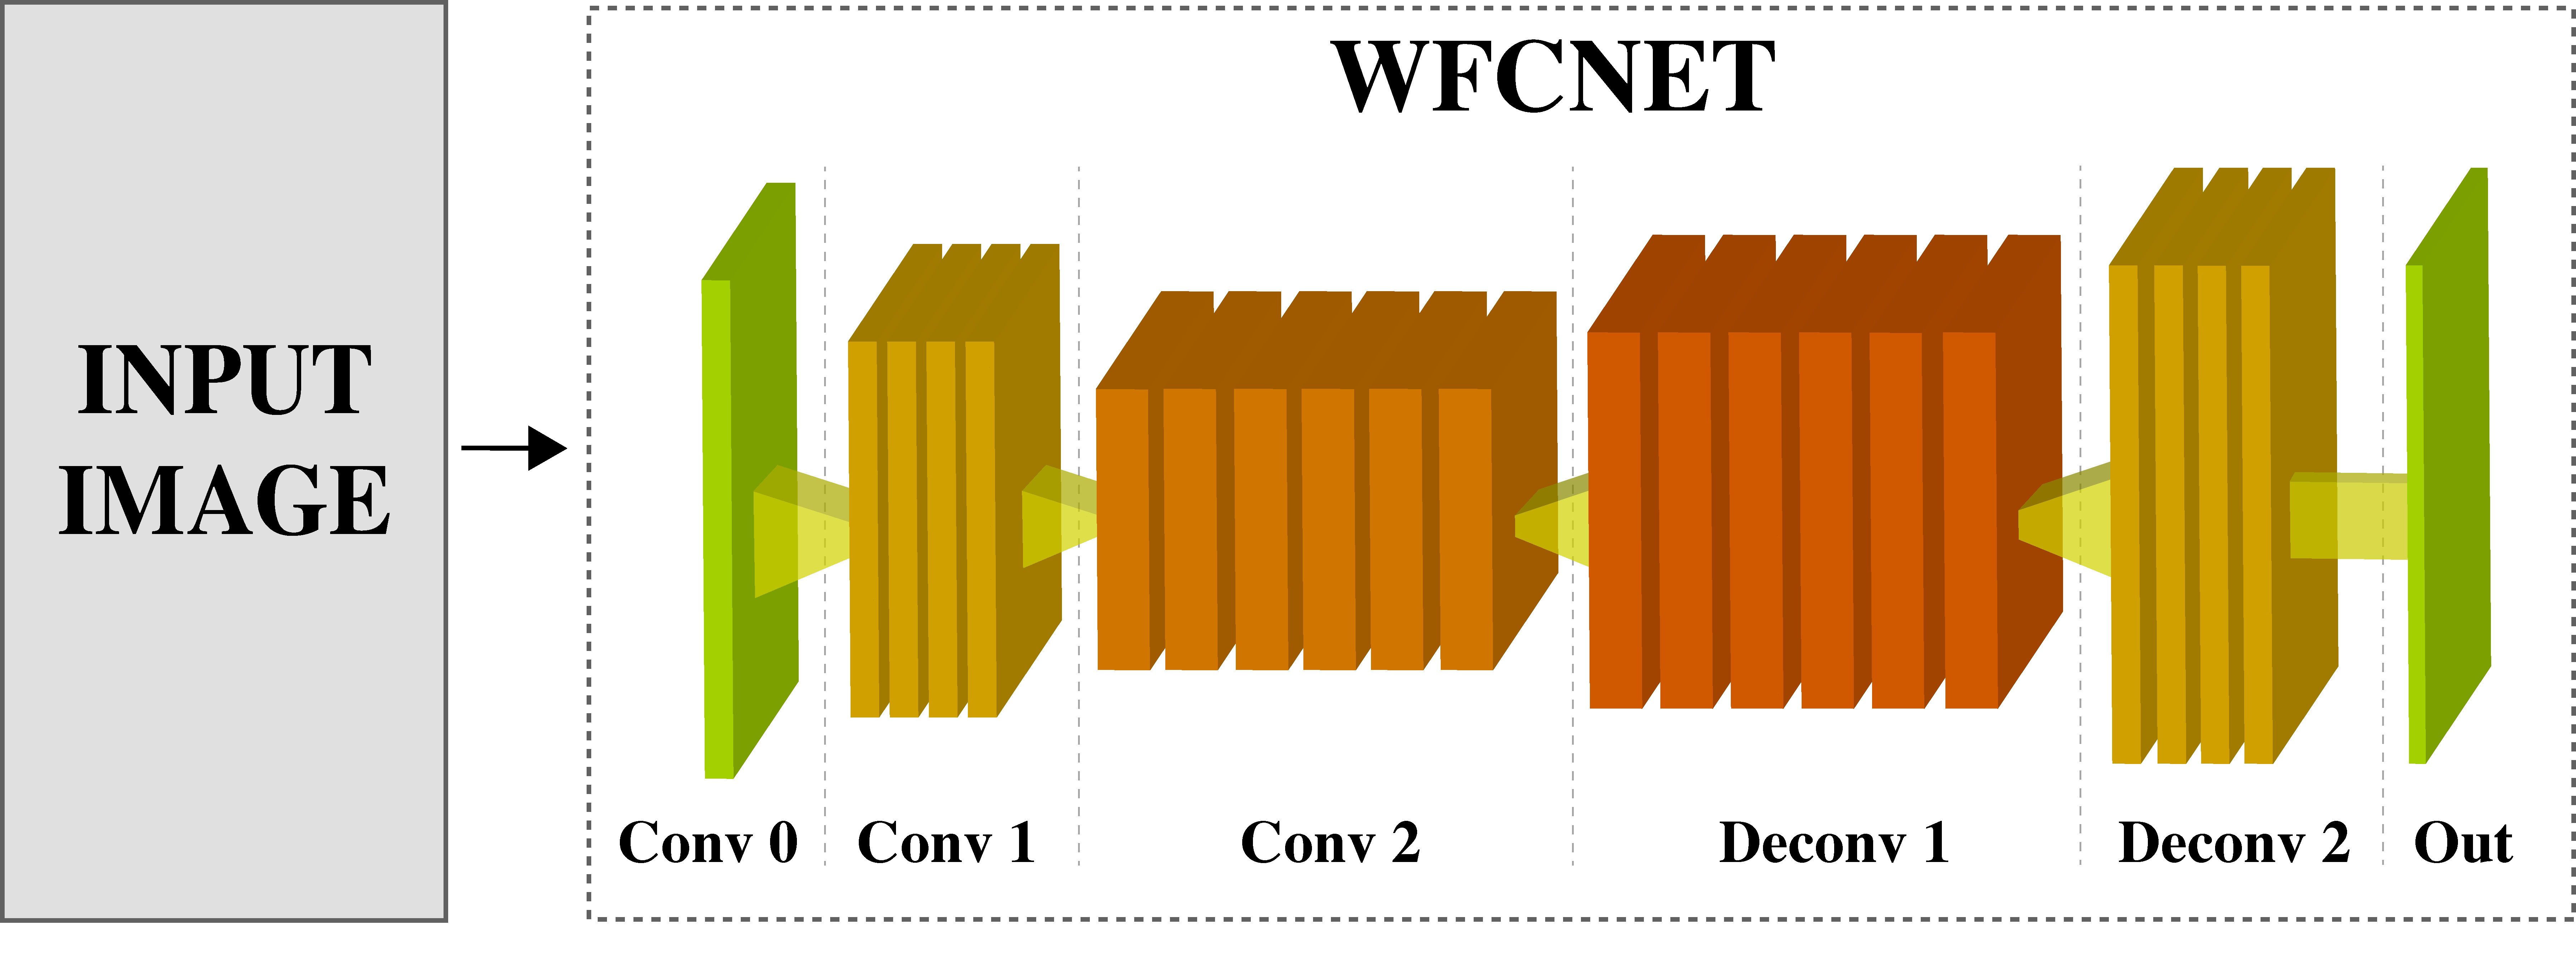
\includegraphics[height=0.40\textheight]{../schemi/training_WFC1}
\end{figure}
 
\end{frame}

\begin{frame}
\frametitle{Training WFCNet 2/2}

\begin{figure}
\centering
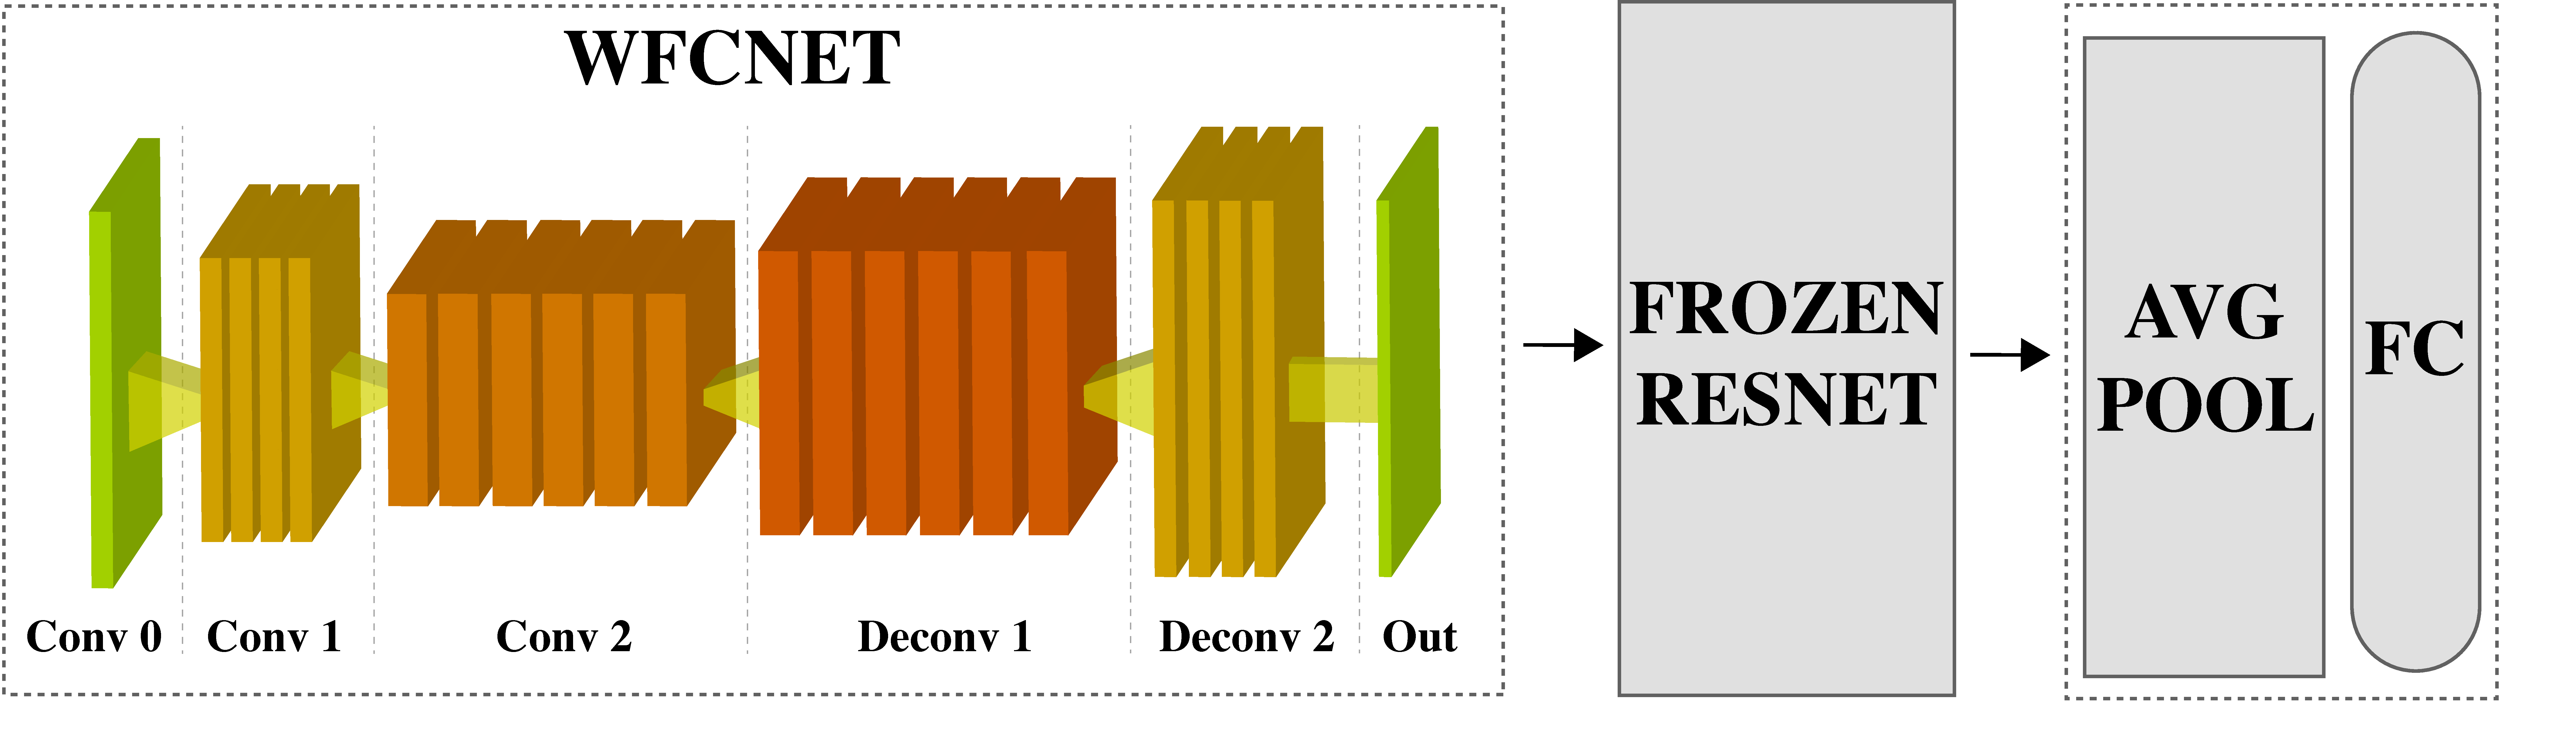
\includegraphics[height=0.40\textheight]{../schemi/training_WFC2}
\end{figure}
 
\end{frame}

\begin{frame}
\frametitle{Colorized Blocks}

\begin{figure}
\centering
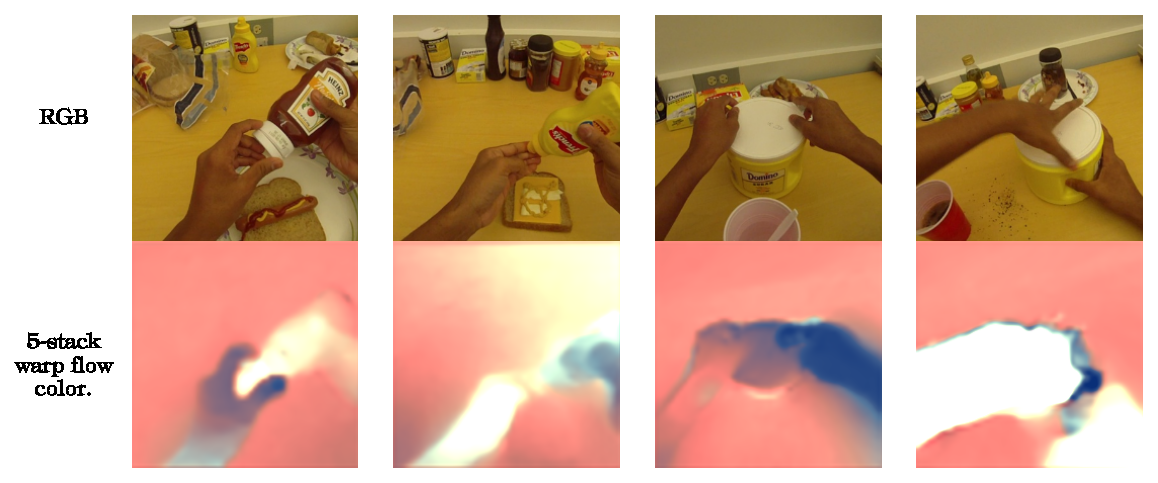
\includegraphics[height=0.50\textheight]{../schemi/wfcnet_color_img}
\end{figure}
 
\end{frame}

\begin{frame}
\frametitle{Single Input 1/2}

Basic features:
\begin{itemize}
\item A \textbf{WFCNet} to infer \textbf{RGB warp flow} frames;
\item A \textbf{ResNet}, with an attention mechanism implemented, \textbf{trained on ImageNet};
\item A \textbf{ConvLSTM} to encode the \textbf{temporal correlations} between the spatial maps; %funziona meglio rispetto alla LSTM perchè 
\item An \textbf{Average Pooling} layer and a \textbf{FC} layer;
\item Due to the kind of problem, i.e classification, a \textbf{Cross Entropy Loss is used};
\end{itemize}
 
\end{frame}

\begin{frame}
\frametitle{Single Input 2/2}

\begin{figure}
\centering
\includegraphics[width=\textwidth]{../schemi/single_stream}
\end{figure}
 
\end{frame}

\begin{frame}
\frametitle{Two Input 1/2}
Limitations of single input:
\begin{itemize}
\item \textbf{The warp flow alone is not sufficient} to achieve high results;
\item \textbf{The warp flow} is not generated with special measurement equipment, so it \textbf{represent a simple domain projection};
\item The \textbf{appearance} is \textbf{discarded};
\end{itemize}

Solution:
\begin{itemize}
\item \textbf{Analyze both} warp flow and RGB frames
\item \textbf{Unique backbone} with \textbf{two attention mechanisms}, one for warp flow and one for RBG;
\end{itemize}
\end{frame}

\begin{frame}
\frametitle{Two Input 2/2}

\begin{figure}
\centering
\includegraphics[width=\textwidth]{../schemi/two_stream_img}
\end{figure}
 
\end{frame}
  
\section{Results}

\begin{frame}
\frametitle{Overview} 
	\tableofcontents[currentsection]
\end{frame}

\begin{frame}
\frametitle{Results 1/2}

	{ \footnotesize 
	\begin{columns}[c]
		\begin{column}{.65\textwidth}
			\begin{itemize}
				\item RGB Network \\
				\vspace*{8pt}
				\begin{tabular}{l|r}
					Network & Mean Val. Acc. \\
					\hline
					RGB w/ NOCAM @ 7 & 54.31\% \\
					RGB w/ CAM @ 7 & 59.19\% \\
					RGB w/ NEW A.M. @ 7 & 59.90\% \\
					\hline
					RGB w/ NOCAM @ 16 & 56.32\% \\
					RGB w/ CAM @ 16 & 66.66\% \\
					RGB w/ NEW A.M. @ 16 & 65.51\% \\
				\end{tabular}
			\item RGB Network w/ MS task \\
			\vspace*{8pt}
			\begin{tabular}{ll|r}
				Type & Frames & Best Acc. \\
				\hline
				Classification & 7 & 60.34\% \\
				Classification & 16 & 68.97\% \\
				Regression & 7 & 61.21\% \\
				Regression & 16 & 68.10\% \\
			\end{tabular}
			\end{itemize}
		\end{column}
		\begin{column}{.7\textwidth}
				\begin{itemize}
					\item Temporal Network \\
					\vspace*{8pt}
					\begin{tabular}{l|r}
						& Mean Val. Acc. \\
						\hline
						1 Stack of 5 & 40.52\% \\
						5 Stacks of 5 & 48.85\% \\
					\end{tabular}
				\item Two stream \\
				\vspace*{8pt}
				\begin{tabular}{l|r}
					Frames & Mean Val. Acc. \\
					\hline
					7 & 68.90\% \\
					16 & 75\%
				\end{tabular}
				\end{itemize}
			\end{column}
	\end{columns}
	}

\end{frame}

\begin{frame}
	\frametitle{Results 2/2}
	
	{ \footnotesize 
		\begin{columns}[c]
			\begin{column}{\textwidth}
				\begin{itemize}
					\item Single input \\
					\vspace*{8pt}
					\begin{tabular}{l|r}
						Network & Val. Accuracy \\
						\hline
						WFCNet single -> RGBNet @ 7 & 26.43\% \\
						WFCNet single -> RGBNet @ 14 & 28.16\% \\
						\hline
						WFCNet stack of 5 -> RGBNet @ 7 & 35.34\% \\
						WFCNet stack of 5 -> RGBNet @ 14 & 33.04\% \\
					\end{tabular}
					\item Two input \\
					\vspace*{8pt}
					\begin{tabular}{l|rr}
						Network & Stage 1 & Stage 2 \\
						\hline
						Stack of 5 + RGB @ 7 & 52.58\% & 63.22\% \\
						Stack of 5 + RGB @ 14 & 60.34\% & 71.83\% \\
					\end{tabular}
				\end{itemize}
			\end{column}
		\end{columns}
	}
	
\end{frame}
     
\begin{frame}
\frametitle{References}
   \begin{thebibliography}{9}
	\bibitem{photos}
		Caroline Cakebread
		\newblock “People will take 1.2 trillion digital photos this year — thanks to smartphones”
		\newblock Businessinsider.com, 1 September 2017
		\newblock Available at: https://www.businessinsider.com/12-trillion-photos-to-be-taken-in-2017-thanks-to-smartphones-chart-2017-8?IR=T
   \end{thebibliography}
\end{frame}

\begin{frame}
\centering
\frametitle{The End}
\Huge Thank you for your attention!
\break
\break
\break
\break
\large Nicolò Bertozzi
\break
Francesco Bianco Morghet
\break
\break
Aid of WFCNet for FPAR Task | MLDL
\break
13 July 2020
\end{frame}

\end{document}